\documentclass[12pt,a4paper]{book}
\usepackage[utf8]{inputenc}
\usepackage[portuguese]{babel}
\usepackage[T1]{fontenc}
\usepackage{amsmath}
\usepackage{amsfonts}
\usepackage{amssymb}
\usepackage{graphicx}
\usepackage{color}
\usepackage{enumitem}

\newtheorem{example}{Exemplo}
\newtheorem{remark}{Observação}

\usepackage[left=3cm,right=2cm,top=3cm,bottom=2cm]{geometry}
\title{Matemática Aplicada e Computacional}
\author{Eduardo José de Oliveira}

\newcommand{\todo}[1]{
	{\color{red}#1}
}

\begin{document}


%
%
%
\chapter{Introdução}

As fases na resolução de problemas em matemática aplicada e computacional que surgem nas mais diversas áreas do conhecimento, de modo geral, podem ser representadas da seguinte maneira:

\begin{figure}[h]
	\centering
	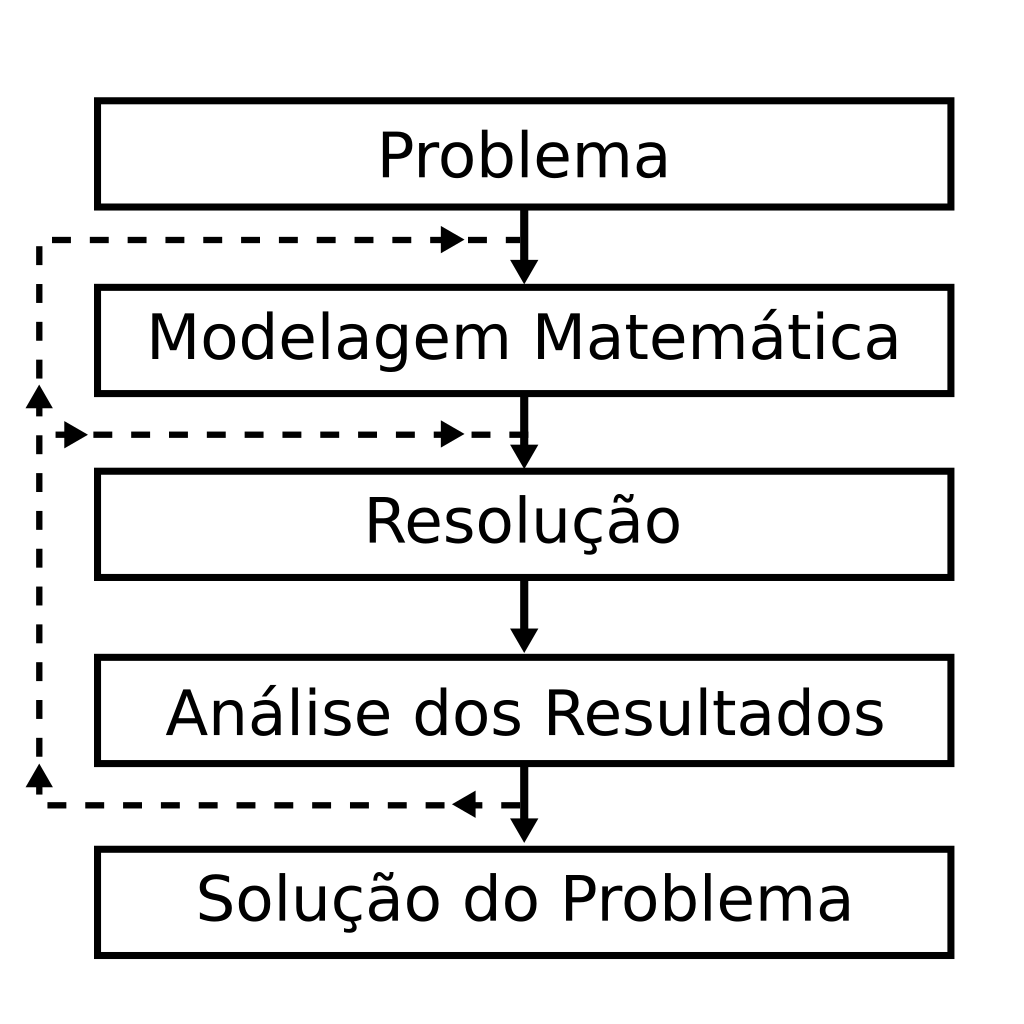
\includegraphics[scale=0.2]{figuras/figura_001}
	\caption{Fluxograma das fases na resolução de problemas em Matemática Aplicada e Computacional.}
\end{figure}

A primeira fase consiste basicamente em definir corretamente o problema a ser solucionado. A fase da modelagem matemática é onde ocorre a construção ou definição do modelo matemático que irá descrever o comportamento do problema em questão. Na fase de resolução são definidos e implementados os métodos para obtenção da solução do problema.

A análise dos resultados tem por finalidade verificar os resultados obtidos na resolução do problema. Se o resultado for satisfatório aceitamos a solução do problema, caso contrário, deve-se procurar outros métodos ou refazer a modelagem matemática.

%
%
%
\chapter{Principais erros na resolução de um problema}

Na resolução de um problema os erros podem surgir em cada fase. A seguir apresentamos os principais:

\section{Erros na fase do problema}

Não definir corretamente o problema é um erro grave que pode levar a falsos resultados.

\section{Erros na modelagem matemática}

O modelo matemático para um problema real deve representar o fenômeno que ocorre no mundo físico, porém, nem sempre é fácil. Normalmente são necessárias simplificações no modelo físico para se obter um modelo matemático (tratável) que fornecerá uma solução para o problema. Essas simplificações se constituem em fonte de erros, o que pode acarretar na necessidade de reformular o modelo matemático adotado.

\begin{example}
	Um matemático quer determinar a altura de um edificio dispondo de uma esfera de metal, um cronômetro e a equação $s=s_0+v_0 t+ \frac{1}{2}at^2$. Para isso, ele sobe no topo do edificio e solta a esfera de metal anotando o tempo até a mesma tocar o solo, ou seja, 3 segundos.
	
	\begin{figure}[h]
		\centering
		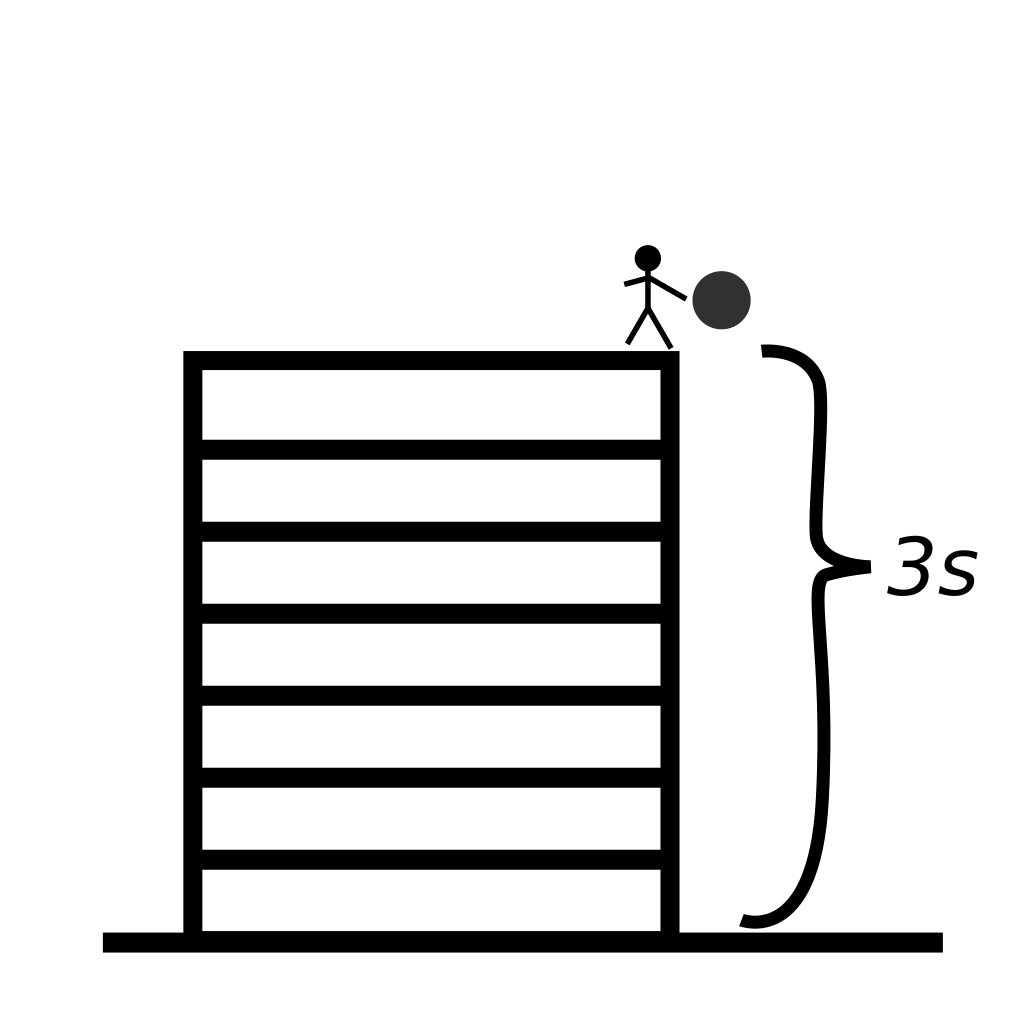
\includegraphics[scale=0.15]{figuras/figura_002}
	\end{figure}
	
	Logo, tem-se $s=s_0+v_0 t+\frac{1}{2}at^2=0+0\cdot 3 + \frac{1}{2}\cdot 9,8 \cdot 3^2=44,1$ m.
	
	Esse resultado é confiável?
	
	Provavelmente não, pois o modelo matemático utilizado não considera outras variáveis relevantes como, por exemplo, a resistência do ar, a velocidade do vento dentre outras.
	
	Além disso, há outro fato que pode influenciar diretamente a precisão na leitura do cronômetro, pois uma pequena variação nessa leitura pode acarretar uma grande variação no cálculo da altura do edificio. Se o tempo medido fosse de 3,5 segundos ao invés de 3 segundos, a altura do edificio seria calculada em 60,025 m. Ou seja, uma variação de 16,67\% na leitura do cronômetro ocasiona uma variação de 36,11\% no cálculo da altura do edifício.
	
	Logo pode-se notar a influência que o modelo matemático e a precisão dos dados de entrada exercem sobre a confiabilidade dos resultados.
\end{example}

\begin{remark}
	Durante a aula, foi proposta uma atividade semelhante em que, utilizando o cronômetro dos celulares e uma bolinha, em duplas, realizando procedimento parecido com o do exemplo, os alunos deveriam estimar a altura da porta da sala de aula.
\end{remark}

\section{Erros na resolução}

Esses erros podem ocorrer na representação de números, na conversão da base e também nos arredondamentos.

Na representação de números, considere o cálculo da área de uma circunferência de raio 100 m, onde utilizaremos os seguintes valores para $\pi$:
\begin{enumerate}[label=\Alph*]
	\item $\pi=3,14\Longrightarrow A=31.400 m^2$.
	\item $\pi=3,1416\Longrightarrow A=31.416 m^2$.
	\item $\pi=3,141592654\Longrightarrow A=31.415,93 m^2$.
\end{enumerate}

A representação de um número depende da base escolhida ou disponível na maquina em uso (computador, calculadora) e do número máximo de dígitos usados na sua representação.

O número $\pi$ não pode ser representado, através de um número finito de dígitos decimais. Neste exemplo utilizou-se três valores para $\pi$, sendo que para cada valor foi encontrado um resultado diferente para a área da circunferência. O erro neste exemplo depende exclusivamente da aproximação escolhida para $\pi$. Qualquer que seja a circunferência, a sua área nunca será obtida exatamente, uma vez que $\pi$ é um número irracional.

Qualquer cálculo que envolva números que não podem ser representados através de um número finito de dígitos não fornecerá como resultado um valor exato. Quanto maior o número de dígitos utilizados, maior será a precisão obtida. Por isso, a melhor aproximação, neste exemplo, para o valor da área da circunferência é quando $\pi=3,141592654$ (caso (c)).

Na conversão de base pode ocorrer que um número tenha representação finita em uma base e não finita em outra base. Por exemplo, o número 0,6 na base decimal é representado pelo número 0,10011001$\dots$ na base 2, isto é:
$$
	(0,6)_{10}=(0,10011001\dots)_{2}
$$

É usual representar e realizar operações com números na base 10 (decimal), mas um número real pode ser representado em qualquer base. Um computador, normalmente, opera no sistema binário, ou seja, base 2.

Em relação ao arredondamento, observe que na interação entre usuário e o computador que opera na base binária, ocorre o seguinte: os dados de entrada são enviados ao computador pelo usuário no sistema decimal e toda essa informação é convertida para a base binária pelo computador e as operações são efetuadas nessa base. Os resultados obtidos no sistema binário são convertidos para o sistema decimal e transmitidos ao usuário.

Todo esse processo de conversão de base pode se constituir em uma fonte de erros de arredondamentos que pode afetar os resultados finais dos cálculos na resolução de um problema.

\begin{example}
	Considere os seguintes valores $x_1=0,003815$ e $x_2=1.234.567.890$ e, as operações $(x_1+x_2)-x_2$ e $x_1+(x_2-x_2)$. Temos os seguintes resultados:

	\begin{itemize}
		\item \textbf{Calculadora científica (10 digitos):}\hfill
		$$(x_1+x_2)-x_2=(0,003815+1.234.567.890)-1.234.567.890=$$
		$$=1.234.567.890-1.234.567.890=0\text{,}$$
		e, no segundo caso,
		$$x_1+(x_2-x_2)=0,003815+(1.234.567.890-1.234.567.890)=$$
		$$=0,003815+0=0,003815\text{.}$$
	\end{itemize}
	\todo{Complementar o exemplo falando sobre o uso de cálculadoras de celular, linguagens de programação (tamanho máximo de números), etc.}
\end{example}

\end{document}